% !TEX root = ../main.tex
\section{Experiments}
\vspace{-0.1in}
In this section, we show experimental results for our online contextualized few-shot learning
paradigm, using \ourchar{} and \ourroom{} (see Sec.~\ref{sec:benchmark}) to evaluate our model, CPM,
and other state-of-the-art methods. For Omniglot, we apply an 8$\times$8 CutOut~\citep{cutout} to
each image to make the task more challenging. 
% Details about the split information can be found in
% Appendix~\ref{app:data}.

\vspace{-0.1in} \paragraph{Implementation details:} For \ourchar{}, we use the common
4-layer CNN for few-shot learning with 64 channels in each layer. For \ourimg{}, we also use ResNet-12 
with input resolution 84$\times$84~\citep{tadam}. For the \ourroom{}, we resize the input to 
120$\times$160 and use ResNet-12. To represent
the feature of the input image with an attention mask, we concatenate the global average pooled
feature with the attention ROI feature, resulting in a 512d feature vector. For the contextual RNN,
in both experiments we used an LSTM~\citep{lstm} with a 256d hidden state. The best CPM model is
equipped using GAU and cosine similarity for querying prototypes. Logits based on cosine similarity
are multiplied with a learned scalar initialized at 10.0~\citep{tadam}. We include additional
training details in Appendix~\ref{app:exp}.

\vspace{-0.1in}
\paragraph{Evaluation metrics:}
In order to compute a single number that characterizes the learning ability over sequences, we
propose to use \textit{average precision} (AP) to evaluate
both with respect to old versus new and the
specific class predictions.
Concretely, all predictions are sorted by their old vs. new scores, and we compute AP using the area
under the precision-recall curve. A true positive is defined as the correct prediction of a
multi-class classification among known classes. We also compute the ``$N$-shot'' accuracy; i.e., the
average accuracy after seeing the label $N$ times in the sequence. Note that these accuracy scores
only reflect the performance on {\it known} class predictions. All numbers are reported with an
average over 2,000 sequences and for $N$-shot accuracy standard error is also included.
Further explanation of these metrics is in Appendix~\ref{sec:metrics}. 

\vspace{-0.1in}
\paragraph{Comparisons:}
To evaluate the merits of our proposed model, we implement classic few-shot learning and online
meta-learning methods. More implementation and training details of these baseline methods can be
found in Appendix~\ref{app:exp}.
% !TEX root = ../main.tex
\begin{figure}[t]
\vspace{-0.5in}
\centering
\iflatexml
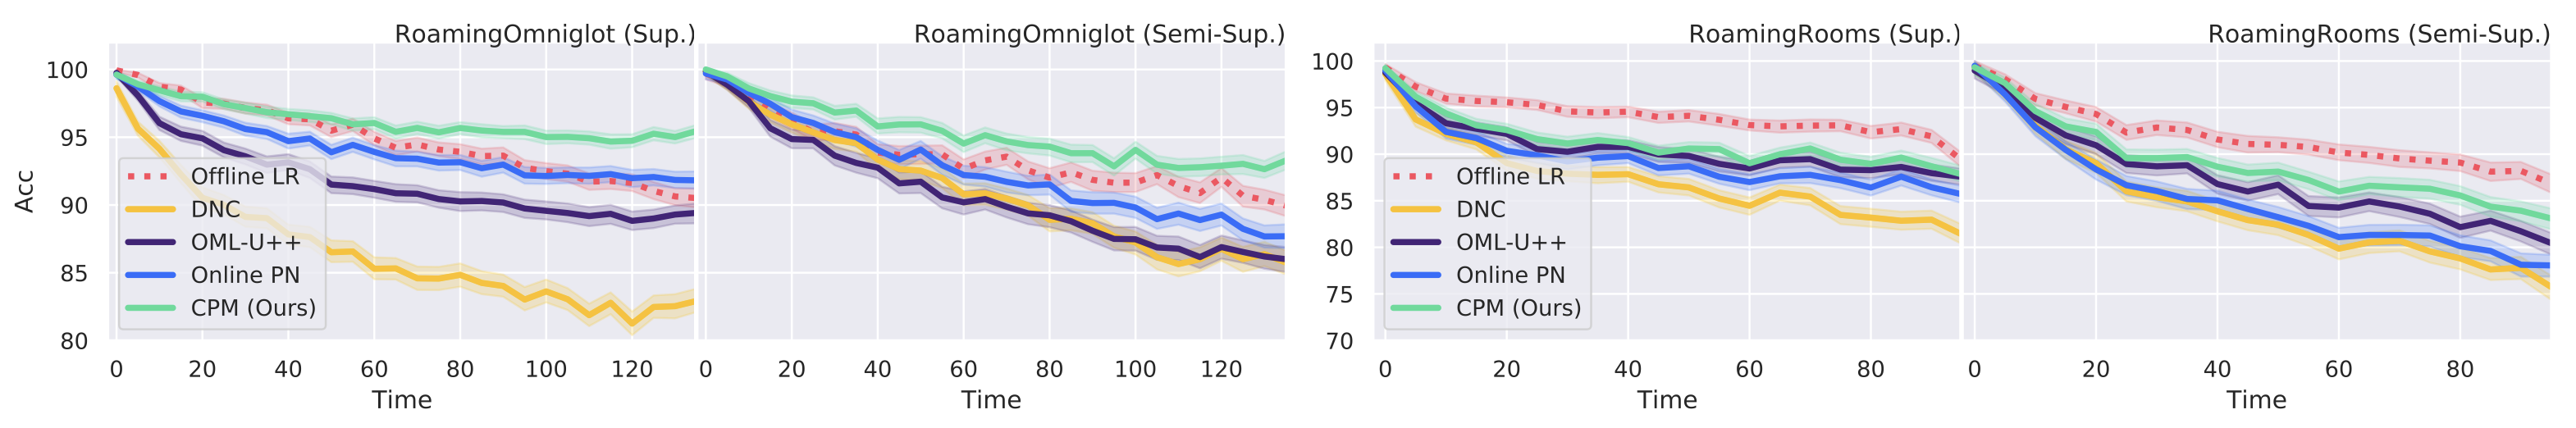
\includegraphics[width=6\linewidth]{figures/acctime_full.png}
\else
\setlength{\tabcolsep}{0pt}
\begin{tabular}{cccc}
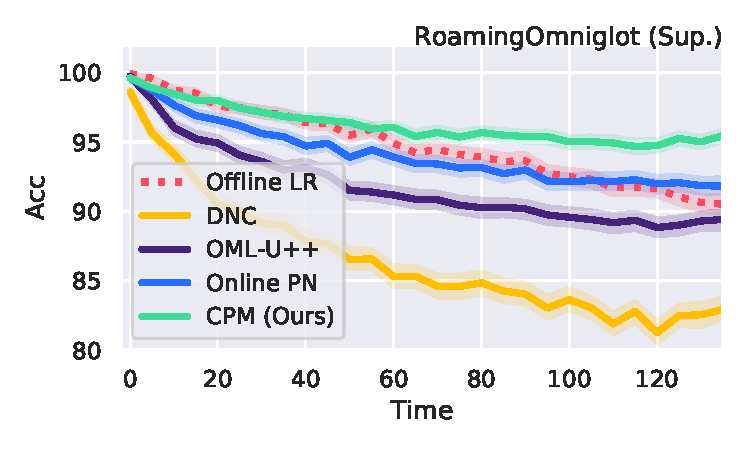
\includegraphics[height=2.4cm,trim={0.3cm 0cm 0.5cm 0},clip]{figures/omniglot-nossl-time.pdf}
&
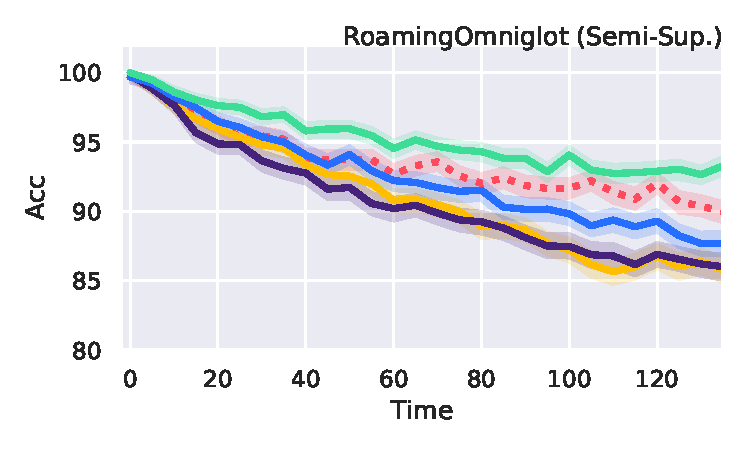
\includegraphics[height=2.4cm,trim={2cm 0cm 0cm 0},clip]{figures/omniglot-ssl-time.pdf}
&
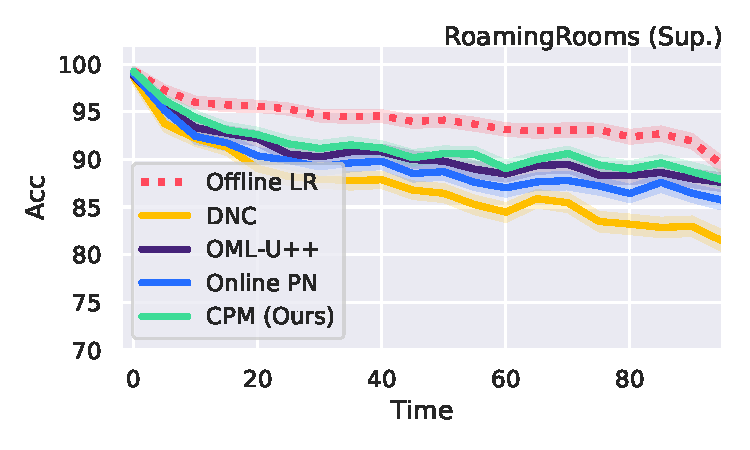
\includegraphics[height=2.4cm,trim={1cm 0cm 0.5cm 0},clip]{figures/matterport-nossl-time.pdf}
&
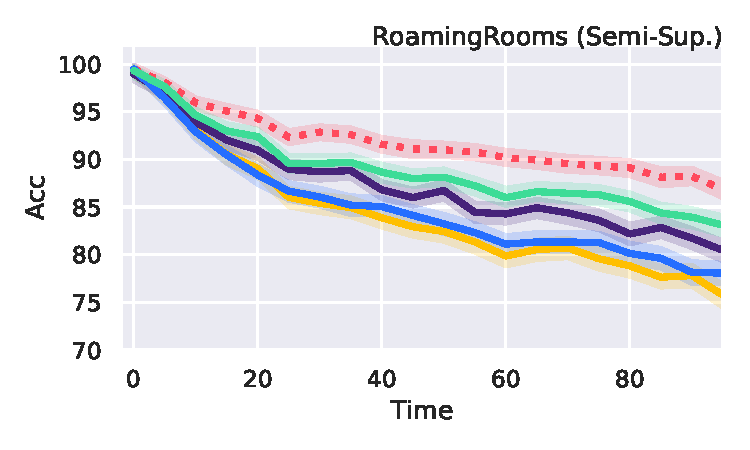
\includegraphics[height=2.4cm,trim={2cm 0cm 0cm 0},clip]{figures/matterport-ssl-time.pdf}
\\
\end{tabular}
\vspace{-0.25in}
\fi
\caption{\textbf{Few-shot classification accuracy over time.} \textbf{Left:} \ourchar{}.
\textbf{Right:} \ourroom{}. \textbf{Top:} Supervised. \textbf{Bottom:} Semi-supervised. An offline
logistic regression (Offline LR) baseline is also included, using pretrained ProtoNet features. It
is trained on all labeled examples except for the one at the current time step.}
\label{fig:acctimefull}
% \vspace{-0.25in}
\end{figure}

% !TEX root = ../main.tex
\begin{figure}[t]
\vspace{-0.1in}
\centering
\iflatexml
    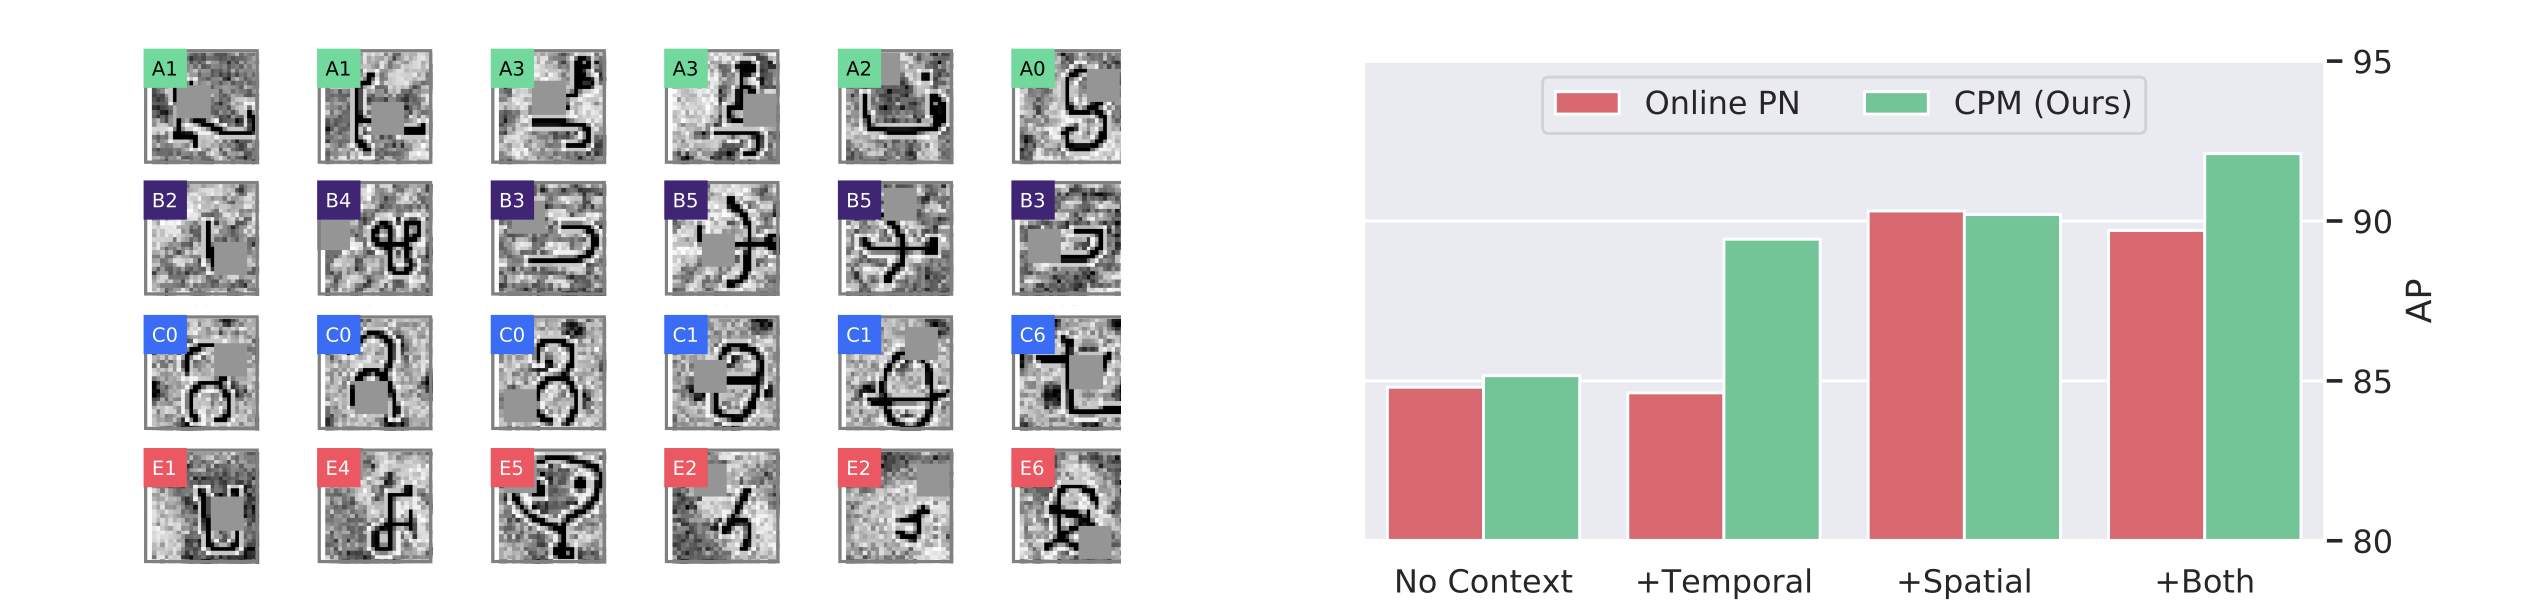
\includegraphics[width=6\linewidth]{figures/spatiotemporal_full.png}
\else
    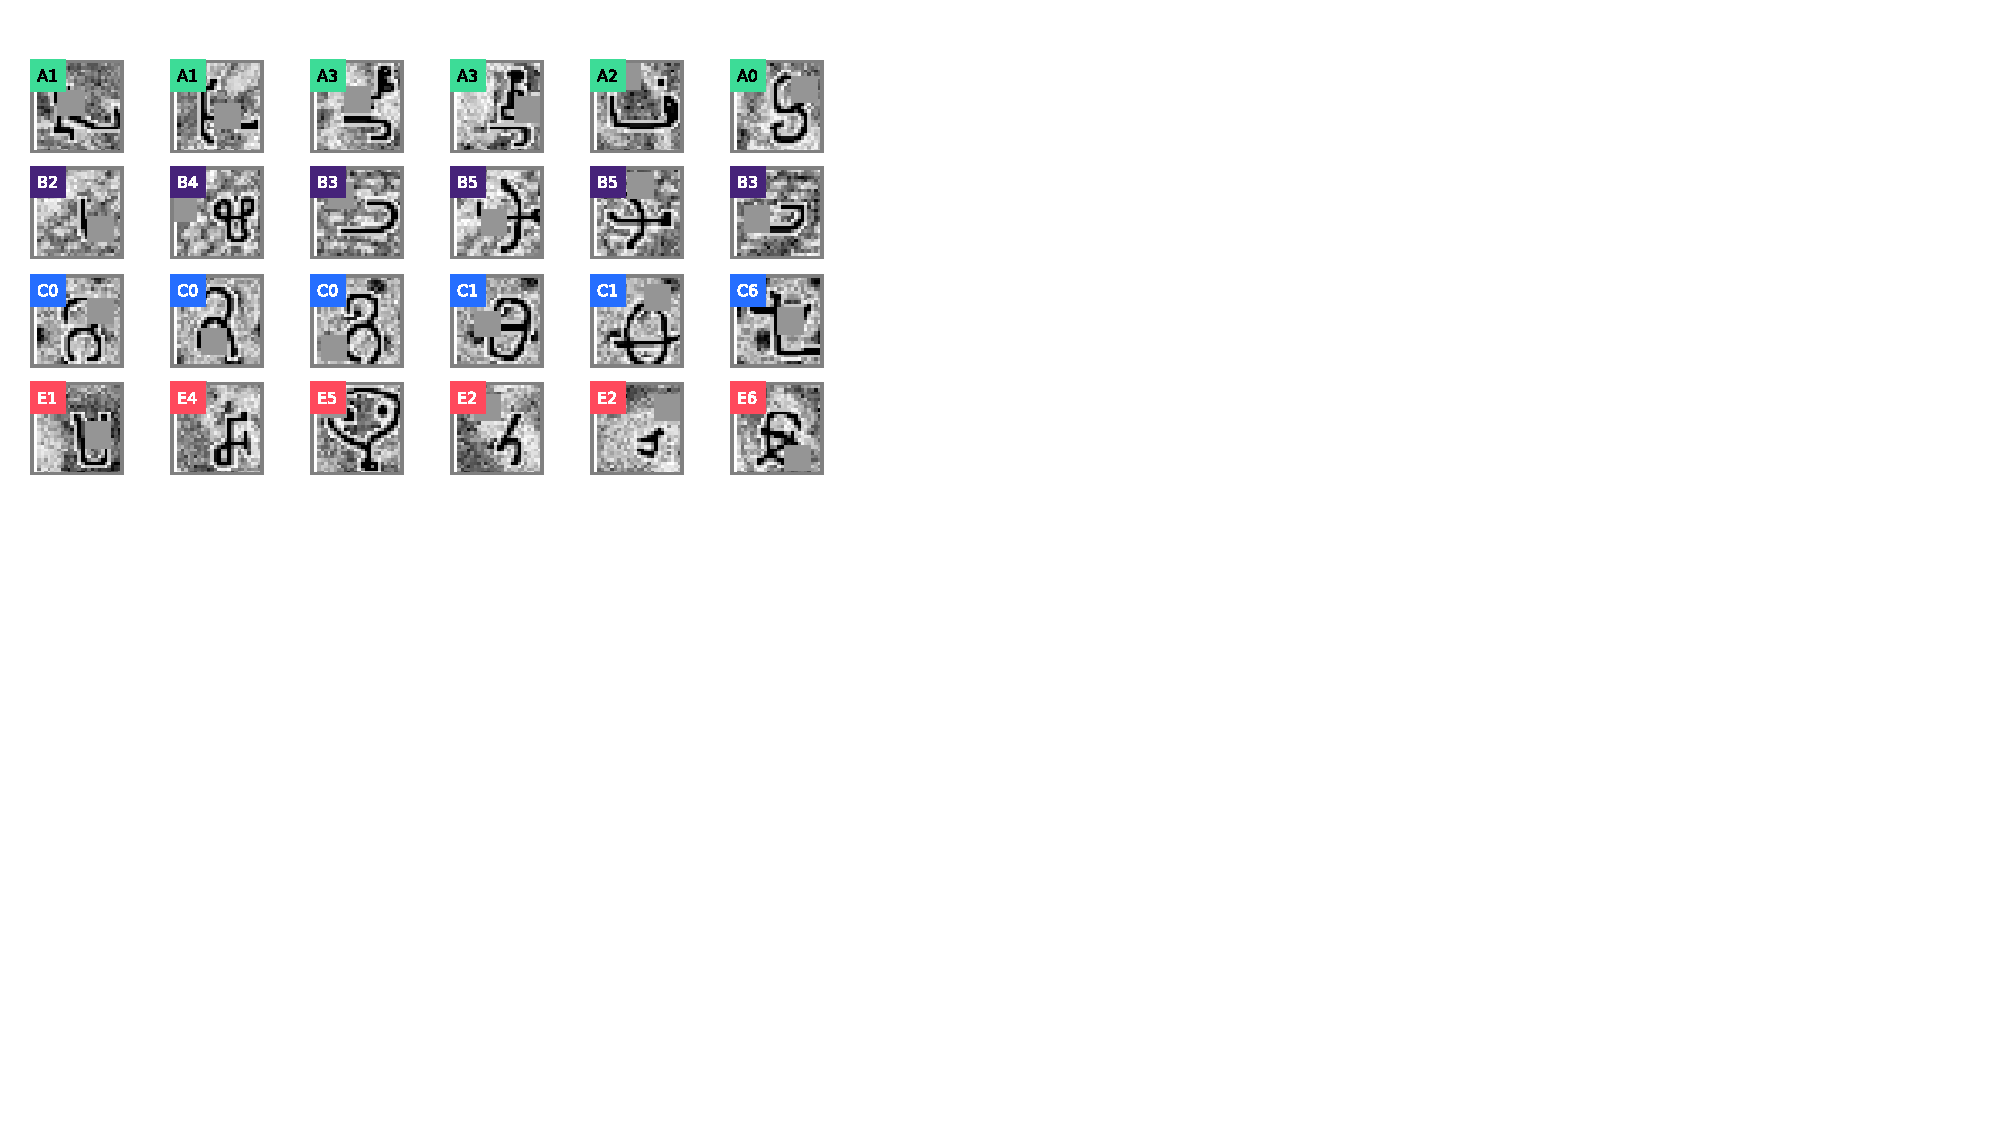
\includegraphics[height=2.8cm,trim={-2.25cm 10cm 20cm 0.5cm},clip]{figures/omniglot-texture.pdf}
    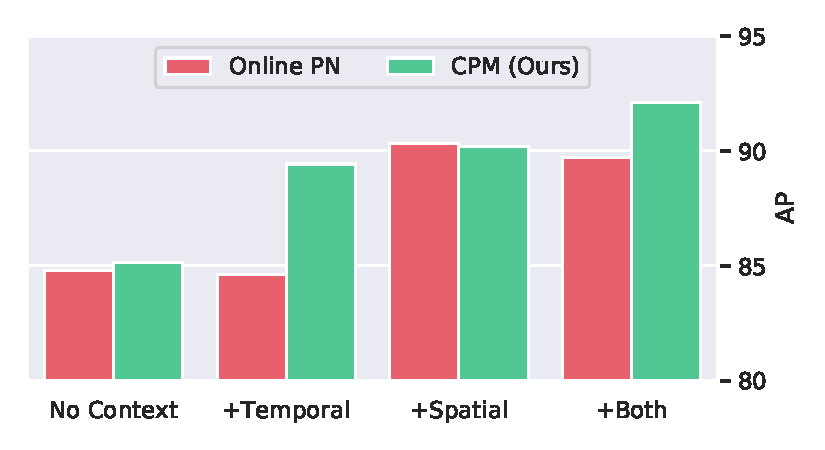
\includegraphics[height=2.8cm,trim={-2.25cm 0 0.5cm 0},clip]{figures/spatiotemporal.pdf}
\fi
\quad
\vspace{-0.2in}
\caption{\textbf{Effect of spatiotemporal context.} Spatiotemporal
context are added separately and together in \ourchar{}, by introducing texture background and
temporal correlation. \textbf{Left:} Stimuli used for spatial cue of the background environment.
\textbf{Right:} Our CPM model benefits from the presence of a temporal context
(``+Temporal'' and ``+Both'')} %, while Spatial context helps both CPM and online ProtoNet.}
\label{fig:spatiotemporal}
% \vspace{-0.1in}
\end{figure}

\vspace{-0.1in}
\iflatexml
\begin{itemize}
    \item \textbf{OML}~\citep{oml}: This is an online version of MAML~\citep{maml}. It performs one
    gradient descent step for each labeled input image, and slow weights are learned via
    backpropagation through time. On top of OML, we added an unknown predictor $\hat{u}_t = 1 -
    \max_k \hat{y}_{t,k}$ \footnote{We tried a few other ways and this is found to be the
    best.} (\textbf{OML-U}). We also found that using cosine classifier without the last layer ReLU
    is usually better than using the original dot-product classifier, and this improvement is denoted
    as \textbf{OML-U++}.
    \item \textbf{LSTM}~\citep{lstm} \& \textbf{DNC}~\citep{dnc}: We include RNN methods for
    comparison as well. Differentiable neural computer (DNC) is an improved version of memory
    augmented neural network (MANN)~\citep{mann}.
    \item \textbf{Online MatchingNet (\OnlineMatchingNet{})}~\citep{matchingnet}, 
    \textbf{IMP (\OnlineIMP{})}~\citep{imp} \&
    \textbf{ProtoNet (\OnlineProtoNet{})}~\citep{protonet}: We used\ the same negative Euclidean distance as the
    similarity function for these three metric learning based approaches.  In particular,
    MatchingNet stores all examples and performs nearest neighbor matching, which can be memory
    inefficient. Note that Online ProtoNet is a variant of our method without the contextual RNN.
\end{itemize}
\else
\begin{itemize}[leftmargin=*]
    \item \textbf{OML}~\citep{oml}: This is an online version of MAML~\citep{maml}. It performs one
    gradient descent step for each labeled input image, and slow weights are learned via
    backpropagation through time. On top of OML, we added an unknown predictor $\hat{u}_t = 1 -
    \max_k \hat{y}_{t,k}$ \footnote{We tried a few other ways and this is found to be the
    best.} (\textbf{OML-U}). We also found that using cosine classifier without the last layer ReLU
    is usually better than using the original dot-product classifier, and this improvement is denoted
    as \textbf{OML-U++}.
    \item \textbf{LSTM}~\citep{lstm} \& \textbf{DNC}~\citep{dnc}: We include RNN methods for
    comparison as well. Differentiable neural computer (DNC) is an improved version of memory
    augmented neural network (MANN)~\citep{mann}.
    \item \textbf{Online MatchingNet (\OnlineMatchingNet{})}~\citep{matchingnet}, 
    \textbf{IMP (\OnlineIMP{})}~\citep{imp} \&
    \textbf{ProtoNet (\OnlineProtoNet{})}~\citep{protonet}: We used\ the same negative Euclidean distance as the
    similarity function for these three metric learning based approaches.  In particular,
    MatchingNet stores all examples and performs nearest neighbor matching, which can be memory
    inefficient. Note that Online ProtoNet is a variant of our method without the contextual RNN.
\end{itemize}
\fi
\iflatexml
\begin{table}[t]
    \centering
    \begin{tabular}{ccccccc|cccccc}
    \toprule
    & \multicolumn{6}{c|}{\textbf{Supervised}} & \multicolumn{6}{c}{\textbf{Semi-Supervised}}\\
    Interval  &   1 - 2&      3 - 5&      6 - 10&     11 - 20&    21 - 50&    51 - 100&
                    1 - 2&      3 - 5&      6 - 10&     11 - 20&    21 - 50&    51 - 100\\
    OPN 1-Shot  &   88.8&       86.9&       85.2&       84.7&	    83.6&	    81.1&
                    90.1&       88.9&	    88.4&	    87.6&	    87.3&	    85.1\\
    CPM 1-Shot  &   \tb{96.1}&  \tb{94.0}&	\tb{93.0}&  \tb{91.6}&	\tb{88.2}&  \tb{84.6}&
                    \tb{95.9}&  \tb{93.8}&  \tb{92.8}&  \tb{91.8}&	\tb{89.4}&  \tb{85.7}\\
    OPN 3-Shot  &   97.2&	    97.1&	    96.6&	    96.7&	    \tb{96.5}&	95.3&
                    97.8&	    97.3&	    97.1&	    \tb{97.8}&	\tb{97.7}&  \tb{96.8}\\
    CPM 3-Shot  &   \tb{98.5}&	\tb{98.2}&	\tb{97.5}&	\tb{97.2}&      95.4&   \tb{95.5}&
                    \tb{98.7}&	\tb{97.5}&	\tb{97.5}&	    96.5&	    96.3&	    92.9\\
    \bottomrule
    \end{tabular}
    \caption{\textbf{Effect of forgetting over a time interval on \ourchar{}.} Average accuracy vs. the number of time steps since the model has last seen the label of a particular class.}
    \label{tab:forgetomniglot}
\end{table}
\else
\begin{table}[t]
\vspace{-0.5in}
    \centering
    \caption{\textbf{Effect of forgetting over a time interval on \ourchar{}.} Average accuracy vs. the number of time steps since the model has last seen the label of a particular class.}
    \vspace{0.1in}
    \resizebox{\textwidth}{!}{
    \begin{tabular}{ccccccc|cccccc}
    \toprule
    & \mc{6}{c}{\bf Supervised} & \mc{6}{c}{\bf Semi-Supervised}\\
    Interval  &   1 - 2&      3 - 5&      6 - 10&     11 - 20&    21 - 50&    51 - 100&
                    1 - 2&      3 - 5&      6 - 10&     11 - 20&    21 - 50&    51 - 100\\
    \midrule
    OPN 1-Shot  &   88.8&       86.9&       85.2&       84.7&	    83.6&	    81.1&
                    90.1&       88.9&	    88.4&	    87.6&	    87.3&	    85.1\\
    CPM 1-Shot  &   \bf{96.1}&  \bf{94.0}&	\bf{93.0}&	\bf{91.6}&	\bf{88.2}&  \bf{84.6}&
                    \bf{95.9}&  \bf{93.8}&  \bf{92.8}&	\bf{91.8}&	\bf{89.4}&	\bf{85.7}\\
    \midrule
    OPN 3-Shot  &   97.2&	    97.1&	    96.6&	    96.7&	    \bf{96.5}&	95.3&
                    97.8&	    97.3&	    97.1&	    \bf{97.8}&	\bf{97.7}&  \bf{96.8}\\
    CPM 3-Shot  &   \bf{98.5}&	\bf{98.2}&	\bf{97.5}&	\bf{97.2}&      95.4&  \bf{95.5}&
                    \bf{98.7}&	\bf{97.5}&	\bf{97.5}&	    96.5&	    96.3&	    92.9\\
    \bottomrule
    \end{tabular}}
    \label{tab:forgetomniglot}
\end{table}
\fi

% !TEX root = ../main.tex
\newcommand{\bgstar}{\beta_t^*, \gamma_t^*}
\newcommand{\bgw}{\beta_t^w$, $\gamma_t^w}
\newcommand{\hrnn}{\bh^{\text{RNN}}}


\iflatexml
    \begin{table}[t]
    \begin{center}
    \begin{tabular}{ccccccc}
    \toprule
    \tb{Method}                   & $\hrnn$ & $\bgstar$ & Metric $\bmm_t$ & GAU  & Val AP      \\
    \midrule                                                            
    \OnlineProtoNet{}             &         &           &                 &      & 91.22       \\
    No $\bh^{\text{RNN}}$         &         &  \yes     & \yes            &      & 92.52       \\
    $\bh^{\text{RNN}}$ only       & \yes    &           &                 &      & 93.48       \\
    No metric $\bmm_t$            & \yes    &  \yes     &                 &      & 93.61       \\
    No $\beta_t^*, \gamma_t^*$    & \yes    &           & \yes            &      & 93.98       \\
    $\bh_t = \bh_t^{\text{RNN}}$  & \yes    &  \yes     & \yes            &      & 93.70       \\
    CPM Avg. Euc                  & \yes    &  \yes     & \yes            &      & 94.08       \\
    CPM Avg. Cos                  & \yes    &  \yes     & \yes            &      & 94.57       \\
    CPM GAU Euc                   & \yes    &  \yes     & \yes            & \yes & 94.11       \\
    CPM GAU Cos                   & \yes    &  \yes     & \yes            & \yes & \tb{94.65}  \\
    \bottomrule
    \end{tabular}
    \end{center}
    \caption{Ablation of CPM architectural components on \ourchar{}}
    \label{tab:ablation} 
    \end{table}

    \begin{table}[t]
    \begin{center}
    \begin{tabular}{cccccccc}
    \toprule
    \tb{Method}         & RNN   & Prototype & $\bgw$ & GAU  & Val AP     \\
    \midrule                                                                                   
    \OnlineProtoNet{}   &       &           &        &      & 90.83      \\
    \OnlineProtoNet{}   &       &  \yes     &        &      & 89.10      \\
    \OnlineProtoNet{}   &       &  \yes     & \yes   &      & 91.22      \\
    CPM                 &       &           &        &      & 92.57      \\
    CPM                 &  \yes &           &        &      & 93.16      \\
    CPM                 &  \yes &  \yes     &        &      & 93.20      \\
    CPM                 &  \yes &  \yes     & \yes   &      & 94.08      \\
    CPM                 &  \yes &  \yes     & \yes   & \yes & \tb{94.65} \\
    \bottomrule
    \end{tabular}
    \end{center}
    \caption{Ablation of semi-supervised learning components on \ourchar{}}
    \label{tab:ablationssl}
    \end{table}
\else
    \begin{table}[t]
    \vspace{-0.1in}
    \begin{minipage}[t]{0.45\textwidth}
    \begin{small}
    \caption{Ablation of CPM architectural components on \ourchar{}}
    \begin{center}
    \label{tab:ablation}
    \resizebox{!}{1.4cm}{
    \begin{tabular}{ccccccc}
    \toprule
    \tb{Method}                   & $\hrnn$ & $\bgstar$ & Metric $\bmm_t$ & GAU  & Val AP      \\
    \midrule                                                            
    \OnlineProtoNet{}             &         &           &                 &      & 91.22       \\
    No $\bh^{\text{RNN}}$         &         &  \yes     & \yes            &      & 92.52       \\
    $\bh^{\text{RNN}}$ only       & \yes    &           &                 &      & 93.48       \\
    No metric $\bmm_t$            & \yes    &  \yes     &                 &      & 93.61       \\
    No $\beta_t^*, \gamma_t^*$    & \yes    &           & \yes            &      & 93.98       \\
    $\bh_t = \bh_t^{\text{RNN}}$  & \yes    &  \yes     & \yes            &      & 93.70       \\
    CPM Avg. Euc                  & \yes    &  \yes     & \yes            &      & 94.08       \\
    CPM Avg. Cos                  & \yes    &  \yes     & \yes            &      & 94.57       \\
    CPM GAU Euc                   & \yes    &  \yes     & \yes            & \yes & 94.11       \\
    CPM GAU Cos                   & \yes    &  \yes     & \yes            & \yes & \tb{94.65}  \\
    \bottomrule
    \end{tabular}
    }
    \end{center}
    \end{small}
    \end{minipage}
    \hfill
    \begin{minipage}[t]{0.45\textwidth}
    \caption{Ablation of semi-supervised learning components on \ourchar{}}
    \begin{small}
    \begin{center}
    \label{tab:ablationssl}
    \resizebox{!}{1.4cm}{
    \begin{tabular}{cccccccc}
    \toprule
    \tb{Method}         & RNN   & Prototype & $\bgw$ & GAU  & Val AP     \\
    \midrule                                                                                   
    \OnlineProtoNet{}   &       &           &        &      & 90.83      \\
    \OnlineProtoNet{}   &       &  \yes     &        &      & 89.10      \\
    \OnlineProtoNet{}   &       &  \yes     & \yes   &      & 91.22      \\
    CPM                 &       &           &        &      & 92.57      \\
    CPM                 &  \yes &           &        &      & 93.16      \\
    CPM                 &  \yes &  \yes     &        &      & 93.20      \\
    CPM                 &  \yes &  \yes     & \yes   &      & 94.08      \\
    CPM                 &  \yes &  \yes     & \yes   & \yes & \tb{94.65} \\
    \bottomrule
    \end{tabular}
    }
    \end{center}
    \end{small}
    \end{minipage}
    \vspace{-0.1in}
    \end{table}
 \fi


\vspace{-0.1in}
\paragraph{Main results:} Our main results are shown in Table~\ref{tab:omniglot}, 
\ref{tab:matterport} and \ref{tab:imagenet}, including both supervised and semi-supervised settings. Our approach achieves
the best performance on AP consistently across all settings. Online ProtoNet is a direct comparison
without our contextual RNN and it is clear that CPM is significantly better. Our method is slightly
worse than Online MatchingNet in terms of 3-shot accuracy on the \ourroom{} semisupervised
benchmark. This can be explained by the fact that MatchingNet stores all past seen examples, whereas
CPM only stores one prototype per class. Per timestep accuracy is plotted in
Figure~\ref{fig:acctimefull}, and the decaying accuracy is due to the increasing number of classes
over time. In \ourchar{}, CPM is able to closely match or even sometimes surpass the offline
classifier, which re-trains at each step and uses all images in a sequence except the current one. This is
reasonable as our model is able to leverage information from the current context.

\vspace{-0.1in}
\paragraph{Effect of spatiotemporal context:} To answer the question whether the gain in performance
is due to spatiotemporal reasoning, we conduct the following experiment comparing CPM with online
ProtoNet. We allow the CNN to have the ability to recognize the context in \ourchar{} by adding a
texture background image using the Kylberg texture dataset~\citep{uppsala} (see
Figure~\ref{fig:spatiotemporal} left). As a control, we can also destroy the temporal context by
shuffling all the images in a sequence. We train four different models on dataset controls with or
without the presence of spatial or temporal context, and results are shown in
Figure~\ref{fig:spatiotemporal}. First, both online ProtoNet and CPM benefit from the inclusion of a
spatial context. This is understandable as the CNN has the ability to learn spatial cues, which
re-confirms our  main hypothesis that successful inference of the current context is beneficial to
novel object recognition. Second, only our CPM model benefits from the presence of temporal context,
and it receives distinct gains from spatial and temporal contexts.

\vspace{-0.1in}
\paragraph{Effect of forgetting:} As the number of learned classes increases, we expect the average accuracy to drop. To further investigate this forgetting effect, we measure the average accuracy in terms of the number of time steps the model has last seen the label of a particular class. It is reported in Table~\ref{tab:forgetomniglot} and in Appendix~\ref{sec:additionalresults} Table~\ref{tab:forgetroom}, \ref{tab:forgetimagenet}, where we directly compare CPM and OPN to see the effect of temporal context.
CPM is significantly better than OPN on 1-shot within a short interval, which suggests that the contextual RNN 
makes the recall of the recent past much easier. On \ourimg{}, OPN eventually surpasses CPM on longer horizon, and this can be explained by the fact that OPN has more stable prototypes, whereas prototypes in CPM could potentially be affected by the fluctuation of the contextual RNN over a longer horizon.

\vspace{-0.1in}
\paragraph{Ablation studies:} We ablate each individual module we introduce. Results are shown in
Tables~\ref{tab:ablation} and~\ref{tab:ablationssl}. Table~\ref{tab:ablation} studies different ways
we use the RNN, including the context vector $\bh^{\text{RNN}}$, the predicted threshold parameters
$\beta_t^*,\gamma_t^*$, and the predicted metric scaling vector $\bmm_{t}$. Table~\ref{tab:ablationssl}
studies various ways to learn from unlabeled examples, where we separately disable the RNN update,
prototype update, and distinct write-threshold parameters $\beta^w_t, \gamma^w_t$ (vs. using
read-threshold parameters), which makes it robust to potential mistakes made in
semi-supervised learning. We verify that each component has a positive impact on the performance.
